\section{Back-end}
As seen is Figure \ref{img:architectureprop}, our Back-end is essentially composed by essentially two parts: \textbf{web crawlers/extraction modules}; \textbf{extraction manager} and the \textbf{data miner}, we will write the requirements for each one of the components.

\subsection{Web crawlers}
Each web crawler (or extraction module) must fulfill common requirements that are listed below \footnote{These requirements are agnostic to the \glspl{osn} context}:
\begin{enumerate}
    \item Web crawlers should be able to login with an user account (an \textit{entry point});
    \item Web crawlers should be able to navigate trough the pages of a given \glspl{osn};
    \item Web crawlers must be capable of performing "human" interactions such as click and scroll;
    \item Web crawlers should be able to output a pre defined (agreed and formally defined in the next section) data schema, covering eventual
    exceptions due to privacy limitations;
    \item Web crawlers must be able to perform user extraction with second order depth, from the user entry point perspective (this means that we want to extract user's friends and friends of friends information);
    \item Extraction modules should provide a global extraction method where extraction parameters can be passed from the outside reducing or amplifying scope of extraction as specified from the outside (e.g. under given circumstances we may only need to extract the friends' list or the basic information like name, city and birth date);
    \item Extraction modules must be available to the data miner trough a web API in order to allow remote and distributed extraction. The web API must wrap all the different supported \glspl{osn} being each one accessible trough a different path within the same web API. The extraction web API required specifications are presented next:
    \begin{itemize}
        \item \textbf{GET /api/v1/extraction/\{osn\}} - should return a confirmation message signalizing that API is up and ready for receiving requests;
        \item \textbf{GET /api/v1/extraction/\{osn\}/\{user\_id\}} - should perform full extraction of the user with the \textit{user\_id} in the \textit{osn} ;
        \item \textbf{POST /api/v1/extraction/\{osn\}/\{user\_id\}} - should receive a set of and set of options, that parameterize the extraction and reduce the scope of the extraction for a given \textit{user\_id} within some \textit{osn}.
        \item \textbf{POST /api/v1/extraction/\{osn\}/} - same as the previous but instead of performing extraction for a given \textit{user\_id}, performs it to a set of \textit{user\_ids} performing multiple extractions;
        \item In API version 1 \textbf{osn} must be one of the following: \textbf{facebook}, \textbf{linkedin};
        \item \textbf{user\_id} is a string that uniquely represents the user within a specific \gls{osn}.
    \end{itemize}
\end{enumerate}

\subsection{Extraction Manager}
Below are the extraction manager requirements \footnote{Again, these requirements are agnostic to the \glspl{osn} context}:

\begin{enumerate}
    \item Orchestration of extraction processes scattered trough various hosts: one should be able to define a list of hosts and the number of extraction processes that each host should handle;
    \item Chunk an entry point (that is a set of user identifiers within the \glspl{osn}) in order to delegate different users to different hosts;
    \item Call the extraction endpoints according to the \glspl{osn} from where we need to extract data;
\end{enumerate}

\subsubsection{Extraction pipeline}

\begin{figure}[h!]
\begin{center}
  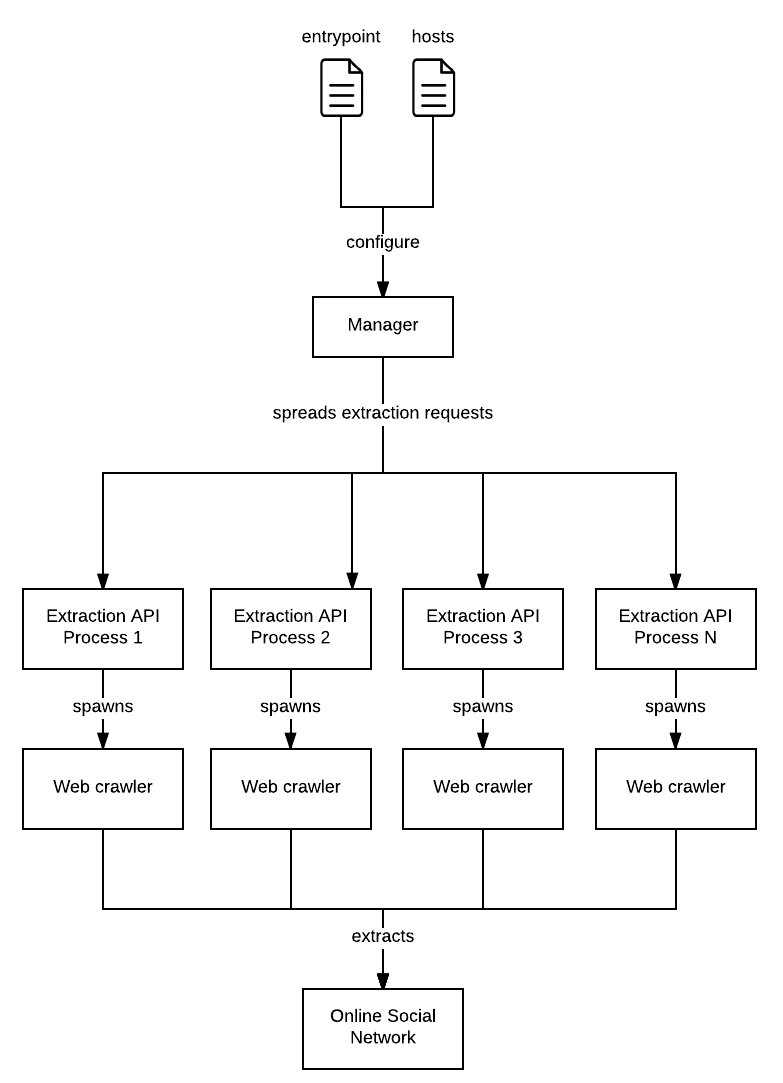
\includegraphics[width=0.7\textwidth]{img/ext-pipeline.png}
\end{center}
\caption{\label{img:extpipeline} Extraction pipeline diagram.}
\end{figure}

Being listed above the requirements for each component we will now draw the specification of what is the expected workflow for data extraction, in Figure \ref{img:extpipeline} we design a pipeline that tries to reflect with maximum detail, the listed requirements. The diagram will not cover the data mining process that is responsible for normalizing data and store it. This diagram is exclusively focused on how we pretend that data extraction is achieved in order to mitigate the slowness of web crawlers.
\\\\
\indent As we can see from Figure \ref{img:extpipeline} we aim to follow a very straight forward process in order to extract information. First we provide an entry point for a given \glspl{osn} (the user the web crawlers will use to log in into the social platform), and a hosts files that describes the resources available for extractions, this is intended to be simply a list of hosts (ip addresses) that have the extraction web API running and awaiting for extraction requests.\\
\indent Next each extraction API instance is responsible for handling a session of some web crawler instance and waits for it to return data so it can give it back to the extraction manager.

\clearpage

\subsection{Data miner}
The data miner simply assures some data treatment before storing it on the database, that said there is a very narrow requirements list for this component:
\begin{enumerate}
\item Receive extraction data and normalize the fields that may need some treatment giving as result a normalized data structure;
\item Store normalized data in the database;
\item Assure that the data schemas (these are presented in the next section) are well defined.
\end{enumerate}

\subsubsection{Data schemas}
Defining data schemas in earlier stages of system specifications will allow us to develop the Front-end and the Back-end simultaneously, we must for that consider that the only source of true when it comes to data structures is a well agreed contract between both parts. The data miner will assure that the next presented schemas are stored in the database. For convenience reasons we will describe the data structures with a JSON like notation.

\subsubsection{Facebook data structure}
\begin{verbatim}
{
    "livesIn": {
        "id": {string},
        "description": {string}
    },
    "life_events": {
        {string}: [{string}]
    },
    "birthDate": {string},
    "likes": {
        {string}: {string}
    },
    "friends": [{string}],
    "relationships": {
        "civil_status": {
            "id": {string},
            "description": {string}
        },
        "family_members": [
            { "id": {string}, "relationship": {string} }
        ]
    },
    "from": {
        "id": {string},
        "description": {string}
    },
    "name": {string},,
    "gender": {string},
    "age": {number},
    "posts": [
        {
            "timestamp": {string},
            "description": {string},
            "author": {string},
            "reactions": {
                "likes": {number},
                "laugh": {number},
                "sad": {number},
                "angry": {number},
                "surprise": {number}
            },
            "comments": {number},
            "shares": {number}
        }
    ]
}
\end{verbatim}

\subsubsection{LinkedIn data structure}
\begin{verbatim}
{
    "id": {string},
    "name": {string},
    "headline": {string},
    "from": {string},
    "summary": {string},
    "experience": [
        {
            "company": {string},
            "position": {string},
            "duration": {
                "count": {number},
                "unit": {string},
                "from": {string},
                "to": {string}"
            }
        }
    ],
    "education": [
        {
            "institution": {string},
            "course": {string},
            "startYear": 2015,
            "endYear": 2017
        }
    ],
    "skills": {
        {string}: 7
    },
    "languages": {
        {string}: {string}
    },
    "projects": [
        {
            "name": {string},
            "date": {string},
            "description": {string}
        }
    ],
    "groups": [
        {string}
    ],
    "following": [
        {string}
    ],
    "connections": [
        {string}
    ]
}
\end{verbatim}

\subsection{Network operations module}
In this section we will list the requirements for the module that is responsible for calculating metrics upon
our stored networks.

...

\begin{enumerate}
    \item max\_clique
    \item enumerate\_all\_cliques
    \item number\_of\_cliques
    \item cliques\_containing\_node

    \item clustering
    \item average\_clustering
    \item max\_clustering

    \item average\_neighbor\_degree

    \item degree\_centrality
    \item closeness\_centrality
    \item betweenness\_centrality
    \item eigenvector\_centrality

    \item triangles

    \item is\_strongly\_connected
    \item number\_strongly\_connected\_components
    \item strongly\_connected\_components

    \item is\_weakly\_connected
    \item number\_weakly\_connected\_components
    \item weakly\_connected\_components

    \item pagerank

    \item shortest\_path
\end{enumerate}
